\documentclass[a4,12pt]{amsart}

\newcounter{chapter}% HACK since amsart has no chapter counter like amsbook
%and there is \numberwithin{theorem}{chapter} in macros.tex,
%seemingly overruled by \numberwithin{theorem}{section} in top.tex

\input macros
\begin{document}
\title{Construction of the circle in UniMath}
{
    \author{Marc Bezem}
    \address{}
    \email{}
    \urladdr{}
}
{
    \author{Ulrik Buchholtz}
    \address{}
    \email{}
    \urladdr{}
}
{
    \author{Daniel R. Grayson}
    \email{danielrichardgrayson@gmail.com}
    \urladdr{http://dangrayson.com/}
}
\date{April 29, 2019}
\maketitle
\numberwithin{theorem}{section}%HACK: executed after \numberwithin{theorem}{chapter}?
%\tableofcontents

\begin{abstract}
We show that the type $\TorZ$ of $\ZZ$-torsors has the dependent universal property of the circle, 
which characterizes it up to a unique homotopy equivalence.  
The construction uses Voevodsky's Univalence Axiom and propositional truncation, 
yielding a stand-alone construction of the
circle not using higher inductive types.
\end{abstract}

\section{Introduction}

In topology it is well known that the classifying space of the group $\ZZ$ of integers is homotopy equivalent to the circle.  In homotopy type
theory and univalent foundations, the {\em types} are the fundamental objects, and they behave much like spaces.  The traditional algebraic
notion of $\ZZ$-torsor yields a category all of whose arrows are isomorphisms, all of whose objects are isomorphic to each other, and a
trivial $\ZZ$-torsor whose automorphism group is $\ZZ$.  Due to univalence, the type $B\ZZ$ of all $\ZZ$-torsors is a connected pointed type
whose fundamental group is $\ZZ$; we may call it the {\em classifying type} of $\ZZ$.  In this paper we show that $B\ZZ$ behaves the way a
circle ought to behave, by establishing that maps from it to other types (or families of types) are freely determined by the destinations of the
base point and the canonical loop at the base point (corresponding to the element $1$ of $\ZZ$.)

As a prerequisite we require working knowledge of homotopy type theory
as described in, for example, the first four chapters of \cite{hottbook}.
One extra piece of knowledge we use here is the \emph{dependent} elimination
principle for propositional truncation, not mentioned in \cite[Ch. 3.7]{hottbook},
and qualified as `not really useful' in \cite[Ch. 6.9]{hottbook}.
\footnote{The dependent elimination principle appears to 
be used later in \cite{hottbook}, though. ULRIK HAS SPOTTED A PLACE}
In \cref{sec:XXX} we give this dependent elimination property some extra
attention, as it is crucial for the computational properties of our construction.

For convenience we give a direct inductive
definition of the set of integers 
in \cref{sec:integers}.  It yields a set
of integers $\zet$, a constant $0:\zet$,
and a successor function $s:\zet\to\zet$
that is an equivalence. We can then define \emph{the 
pointed type of $\zet$-torsors} by
\[
\TorZ\defeq \sum_{(X,f)}\Trunc{(\zet,s)=(X,f)} \text{~with~}
\pt\defeq ((\zet,s),\trunc{\refl{(\zet,s)}}).
\]
Here and below, such pairs $(X,f)$ are of type $\sum_{X:\UU}(X\to X)$.
It is not difficult to see 
that $\pt =_\TorZ \pt$ is equivalent to $\zet$.  To see that, 
begin by observing that every function $f:\zet\to\zet$ commuting with $s$
is propositionally equal to $s^{f(0)}$.  The first projection
acting on $p : \pt =_\TorZ \pt$ gives a path $\mathsf{pr}_1(p) : \zet=\zet$
such that the corresponding transport function $\mathsf{pr}_1(p)_* : \zet\to\zet$
is a bijection commuting with $s$. We evaluate this bijection in $0$.
Let $\ev_0(p) \defeq \mathsf{pr}_1(p)_*(0)$ for all $p : \pt =_\TorZ \pt$,
then $\ev_0 : (\pt =_\TorZ \pt) \to \zet$.  Combining these observations,
using the univalence axiom, one proves that $\ev_0$ is an equivalence.

The preimage of $s(0)$ under the equivalence $\ev_0$ is a
natural generating path of $\pt =_\TorZ \pt$, so we define
${\Zloop}\defeq ev_0^{-1}(s(0))$, which we call the \emph{loop}
of $\TorZ$. Alternatively, we could have obtained $\Zloop$
directly from $s: \zet\equiv\zet$ by applying UA
(with some easy add-ons, e.g., proving that $s$ commutes with itself).

With this in hand, we can formulate a recursion principle for $\TorZ$.
It states that, given a type $A$, an element $a$ of $A$ and a
path $l:a=_A a$, one can construct a function $f:\TorZ\to A$
such that $f(\pt)\jdeq a$ and $\ap{f}(\Zloop)=l$.
(This construction was formalised by Grayson 
in 2014, see \cite{circlerec-Dan}; our construction here uses the 
same basic idea but manages the computations involved in establishing the
induction principle better.)  We call the resulting function
\[
{\rec}_A : \sum_{a:A}(a=a) \to (\TorZ \to A).
\]

The universal property of the circle for $\TorZ$
states that ${\rec}_A$ above is an equivalence, for all types $A$.
In order to prove this universal property one needs an induction
principle, in which $A$ is not a type but a type family over $\TorZ$.
On the basis of Grayson's construction of the recursion principle,
Shulman sketched a possible approach to the induction principle, see \cite{circleind-Mike}. 
Independently of this, but also departing from Grayson's proof of the 
recursion principle, Buchholtz and Bezem found the construction
presented in this paper, which has subsequently been formalized
by Grayson \cite{circleind-Dan,circleind-Dan-theorem} in {\em UniMath}.  

The precise statement of the induction principle is that there is a 
function of the following type, with $\apd{\_}$ from \cite[Ch. 2.3]{hottbook}:

\[
\prod_{A: \TorZ\to\UU}~
\prod_{a: A(\pt)}~
\prod_{l: a=^A_{\Zloop} a}~
\sum_{f: \prod_{z:\TorZ} A(z)}~
\sum_{r: f(\pt)= a}~
{\apd{f}(\Zloop) = r\cto' l \cto r^{-1}}.
\]

Note that $r$ above is a path between two elements of the same fiber $A(\pt)$.
Hence both $r$ and $r^{-1}$ are paths over $\refl{\pt}$ and can be composed with $l$.
To simplify the statement, we use both \emph{left recursive} pathover 
composition $\cto'$ and \emph{right recursive} $\cto$.
If the underlying type theory has propositional truncation with a dependent eliminator 
that computes judgmentally on the point constructor, such as in \cite[Ch. 6.9]{hottbook},
then the same is true for our circle, i.e., the path $r : f(\pt)= a$ above is a reflexivity path.
In that case $r\cto' l \cto r^{-1}$ is judgmentally equal to $l$.   

%The \emph{UniMath} project lacks dependent elimination for propositional truncation, so
The convention in {\em UniMath} is to avoid higher inductive types, and thus
the formalization in \cite{circleind-Dan} is 
somewhat different from the construction presented below.
The formalized construction does not use higher inductive types, nor does it 
%PROOF IN PAPER USES \Trunc AS HIT
depend on the previous existence of a type satisfying the induction principle of the circle. 
However, in a type theory where higher inductive types are admitted,
one can introduce a circle $\Sc$ as a higher inductive type, 
as in \cite[Ch. 6.1]{hottbook}, and it will be equivalent to $\TorZ$. 
The equivalence can be established by observing that $\TorZ$ and $\Sc$ 
are pointed connected types with loop spaces equivalent to $\zet$.
(For the interested reader: apply \cite[Lemma 7.6.2]{hottbook} with $n=-2$
to reduce to action on paths. Then use connectedness to strengthen
this result from embeddings to equivalences. 
Finally, again using connectedness, reduce to the loop spaces
of the respective points, indeed both equivalent to $\zet$.) 

\section{The integers}
\label{sec:integers}

We define the type of integers in one of the many possible ways.

\begin{definition}\label{def:integers}
Let $\zet$ be the inductive type with the following three constructors:
\begin{enumerate}
\item $\zzero: \zet$ for the integer number zero, 
$0 \defeq \zzero$
\item $\zpos: \NN \to \zet$ for positive numbers,
$1 \defeq \zpos(0),\ldots$.
\item $\zneg: \NN \to \zet$ for negative numbers, 
$-1 \defeq \zneg(0),\ldots$
\end{enumerate}
\end{definition}

The \emph{embedding} function $i:\NN\to\zet$ is defined by induction,
setting $i(0)\defeq \zzero$, $i(S(n))\defeq \zpos(n)$.
Like the type $\NN$, the type $\zet$ is a set with decidable equality
and ordering relations,
and we denote its elements often in the usual way as $\ldots,-1,0,1,\ldots$.

One well-known equivalence is \emph{negation} ${-}:\zet\to\zet$, 
also called \emph{complement}, inductively defined by setting 
$-\zzero\defeq \zzero$, 
$-\zpos(n)\defeq \zneg(n)$, 
$-\zneg(n)\defeq \zpos(n)$.
Negation is its own inverse.

The \emph{successor} function $s:\zet\to\zet$ is defined inductively setting 
$s(\zzero)\defeq \zpos(0)$, 
$s(\zpos(n))\defeq \zpos(S(n))$,
$s(\zneg(n))\defeq -i(n)$. For example, we have
$s(-1)\jdeq s(\zneg(0))\jdeq -i(0) \jdeq \zzero \jdeq 0$.
By induction on $n:\NN$ one proves $s(i(n))=i(S(n))$, 
so that one can say that $s$ extends $S$ on the $i$-image of $\NN$. 
From now on we will identify $i(n):\zet$ with $n$,
and $-i(n):\zet$ with $-n$, for all $n:\NN$.

The successor function $s$ is an equivalence.
%It is instructive to depict iterating $s$ in both directions as 
%a doubly infinite sequence containing all integers:
%\[
%\ldots \mapsto \zneg(1) \mapsto \zneg(0) \mapsto \zzero \mapsto \zpos(0) \mapsto \zpos(1) \mapsto \ldots
%\]
The inverse $s^{-1}$ of $s$ is called the \emph{predecessor} function.
We denote the $n$-fold iteration of $s$ as $s^n$, and
the $n$-fold iteration of $s^{-1}$ as $s^{-n}$.

Addition of integers is defined inductively by setting
$z + \zzero\defeq z$, 
$z + \zpos(n)\defeq s^{n+1}(z)$, 
$z + \zneg(n)\defeq s^{-(n+1)}(z)$.
%Again, addition extends $+$ on the $i$-image of $\NN$,
%see \cref{xca:addition-on-Z-and-N}. 
From addition and unary $-$ one can define a binary
\emph{substraction} function setting $z-y \defeq z+(-y)$.

%\begin{xca}\label{xca:addition-on-Z-and-N}
%Show that $i(n+m)=i(n)+i(m)$ for all $n,m:\NN$.
%\end{xca}

Recall the equivalence $\ev_0 : (\pt=_\TorZ \pt)\to\zet$ from the introduction.
We have $\refl{\pt} : \pt=_\TorZ \pt$, as well as the operations
of \emph{path reversal} and \emph{path composition} as defined
in \cite[Ch. 2.1]{hottbook}. These satisfy the laws as stated
and proved in \cite[Lemma 2.1.4]{hottbook}, equipping $\pt=_\TorZ \pt$
with a group structure.
The equivalence $\ev_0$ maps $\refl{\pt}$ via $\id_\zet : \zet\to\zet$ to $0$.
As explained in the introduction, $\ev_0$ maps any $p : \pt=_\TorZ \pt$
via $s^k : \zet\to\zet$ to some $k:\zet$. Since $(s^k)^{-1} = s^{-k}$
and $s^k \circ s^l = s^{k+l}$, $\ev_0$ transports path reversal 
and path composition to negation and addition, respectively.
This means that the entire group structure of $\pt=_\TorZ \pt$
is transported to the usual group structure on $\zet$,
including all the proofs of the group laws in $\zet$.
(The fact that we do not have to reprove the group laws
is one of the benefits of the univalent approach.)


\section{Some induction principles for the integers}
\label{sec:integers-induction}

From the definition of $\zet$ we get the following slightly better induction principle:
Given $P : \zet \to \UU$, to construct elements $h(z) : P(z)$ for every $z : \zet$,
it suffices to give $h(0): P(0)$ and two functions
$f : \prod_{n:\NN}(P(n) \to P(n+1))$ and
$g : \prod_{n:\NN}(P(-n) \to P(-n-1))$, 
see \cref{fig:integers-induction-asymmetric}.

The function $h:\prod_{z:\ZZ}(P(z)$ thus defined satisfies
$h(n+1)\jdeq f(n,h(n))$ and $h(-n-1)\jdeq g(n,h(-n))$ for all $n:\NN$.

\begin{figure}[h]
  \centering
  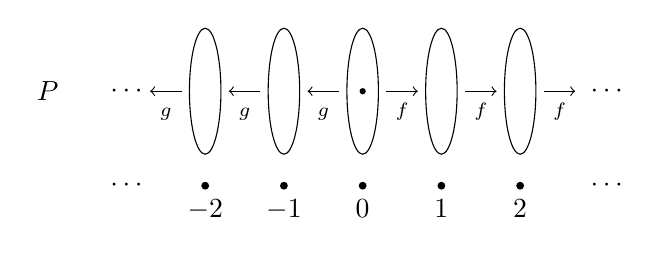
\begin{tikzpicture}
    \foreach \x in {-2,-1,0,1,2} {
      \begin{scope}[shift={(\x,0)}]
        \draw (0,0) ellipse (0.2 and 0.8);
        \node[fill,circle,inner sep=1pt,label=below:{$\x$}] (P\x) at (0,-1.2) {};
      \end{scope}
    }
    \foreach \x in {0,1,2} {
      \begin{scope}[shift={(\x,0)}]
        \draw[->] (0.3,0) -- node[below] {\scriptsize$f\strut$} (0.7,00);
      \end{scope}
    }
    \foreach \x in {-3,-2,-1} {
      \begin{scope}[shift={(\x,0)}]
        \draw[->] (0.7,0) -- node[below] {\scriptsize$g\strut$} (0.3,00);
      \end{scope}
    }
    \node[fill,circle,inner sep=.8pt] at (0,0) {};
    \node at (-4,0) {$P$};
    \node at (-4,-1.4) {$\ZZ$};
    \foreach \x in {-3,3.1} {
      \foreach \y in {0,-1.2} {
        \node at (\x,\y) {$\cdots$};
      }
    }
  \end{tikzpicture}
  \caption{Asymmetric integer induction principle}
  \label{fig:integers-induction-asymmetric}
\end{figure}


It is possible to give a more symmetric, but less general induction principle,
if assume that the functions are equivalences.
In that case we can reorient the $g$'s to point in the same direction as the $f$'s,
so that we just give $f : \prod_{z:\zet}P(z) \equiv P(z+1)$, 
see \cref{fig:integers-induction-symmetric}.

\begin{figure}[h]
  \centering
  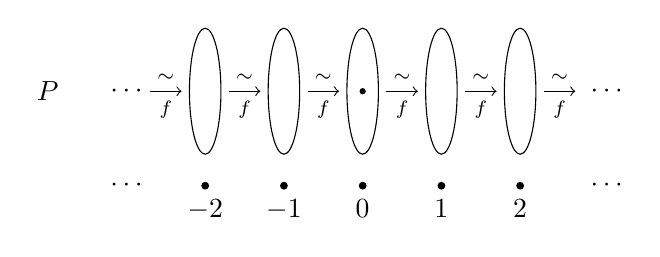
\begin{tikzpicture}
    \foreach \x in {-2,-1,0,1,2} {
      \begin{scope}[shift={(\x,0)}]
        \draw (0,0) ellipse (0.2 and 0.8);
        \node[fill,circle,inner sep=1pt,label=below:{$\x$}] (P\x) at (0,-1.2) {};
      \end{scope}
    }
    \foreach \x in {-3,-2,-1,0,1,2} {
      \begin{scope}[shift={(\x,0)}]
        \draw[->] (0.3,0) -- node[above] {\scriptsize$\sim$} node[below] {\scriptsize$f$} (0.7,00);
      \end{scope}
    }
    \node[fill,circle,inner sep=.8pt] at (0,0) {};
    \node at (-4,0) {$P$};
    \node at (-4,-1.4) {$\ZZ$};
    \foreach \x in {-3,3.1} {
      \foreach \y in {0,-1.2} {
        \node at (\x,\y) {$\cdots$};
      }
    }
  \end{tikzpicture}
  \caption{Symmetric integer induction principle}
  \label{fig:integers-induction-symmetric}
\end{figure}

We shall need that in this case, giving a element $h:\prod_{z:\zet}P(z)$
such that $h(z+1) = f_z(h(z))$ for all $z:\zet$
is in fact equivalent to giving the single element $h(0)$.
We formulate this precisely as follows.

\begin{theorem}\label{thm:integers-univ-symm}
  Let $P : \zet \to \UU$ and $f : \prod_{z:\zet}P(z) \equiv P(z+1)$. The function
  \[
    \varphi : \biggl(\sum_{h:\prod_{z:\zet}P(z)}\prod_{z:\zet}h(z+1) = f_z(h(z))\biggr) \to P(0)
  \]
  that sends $(h,q)$ to $h(0)$ is an equivalence.
\end{theorem}
\begin{proof}
  We prove that the fiber over any $p : P(0)$ is contractible.
  We simplify notations a bit by leaving out the types of $h$ and $q$.
  The fiber $\sum_{(h,q)} h(0)=p$ consists of triples $(h,q,r)$ with $r : h(0) = p$.
  By case distinction, $h$ can (equivalently) be split in three parts $(h_-,h_0,h_+)$
  with $h_0 : P(0)$, $h_+ : \prod_{n:\NN}P(n+1)$,  and $h_- : \prod_{n:\NN} P(-n-1)$. 
  Since $h(0)=p$ only depends on $h_0$ the pair $(h_0,r)$ with  $r : h_0 = p$
  contracts away, so we're left with the type
  \begin{align*}
    \varphi^{-1}(p)
    &\equiv
      \Biggl(\sum_{h_+ : \prod_{n:\NN}P(n+1)}
      \bigl(h_+(0) = f_0(p)\bigr) \\
    &\qquad\qquad\qquad
      \times \biggl(\prod_{n:\NN}h_+(n+1) = f_n(h_+(n))\biggr)\Biggr) \\
    &\quad\times
      \Biggl(\sum_{h_- : \prod_{n:\NN}P(-n-1)}
      \bigl(h_-(0) = f_{-1}^{-1}(p)\bigr) \\
    &\qquad\qquad\qquad
      \times \biggl(\prod_{n:\NN}h_-(n+1) = f_{-n-2}^{-1}(h_-(n))\biggr)\Biggr).
  \end{align*}
  The latter type is contractible, because it is the product of two contractible types,
  each specifying a certain function $h_{\pm}:\prod_{n:\NN}Q_{\pm}(n)$,
  and saying that this function has a certain value at $0$
  and prescribing the values at successors.
  But such a specification is unique by the universal property (induction!) of $\NN$.
\end{proof}
Let us analyze the inverse function produced in the proof.
It maps $p : P(0)$ to a pair whose first component
is the function that takes $z:\zet$ to $f^z(p):P(z)$, where
\begin{alignat*}2
  f^0(p) &\defeq p, && \\
  f^{n+1}(p) &\defeq f_n(f^n(p)),&\quad&\text{for $n:\NN$,} \\
  f^{-n-1}(p) &\defeq f_{-n-1}^{-1}(f^{-n}(p)),&\quad&\text{for $n:\NN$.}
\end{alignat*}


\section{Identifying elements in members of families of types}
\label{sec:pathovers}

In this section we present some addiational results that are needed in the sequel.
% and that cannot be found in \cite{hottbook}.

Let $A : \UU$, $B : A \to \UU$, $a_i:A$, $b_i:B(a_i)$ for $i=1,2$, and $p : a_1 = a_2$.
We are interested in identifications of $b_1$ and $b_2$ relative to this data.
We cannot in general form the type $b_1 = b_2$ as their types may be different.
There are several ways to solve this problem. One of them is to transport $b_1$ along
$p$ and form an identity type in $B(a_2)$. Another way would be to consider
identifications $(a_1,b_1) = (a_2,b_2)$ in $\sum_{x:A} B(x)$ and require that the
action of the first projection on such identifications is equal to $p$. 
These two ways are equivalent.
%The latter way has perhaps been the inspiration of the name `pathover'.
The former way is easier to work with and will be the one we choose here.

\begin{definition}\label{def:pathover}
Let $A : \UU$, $B : A \to \UU$, $a_i:A$, $b_i:B(a_i)$ for $i=1,2$, and $p : a_1 = a_2$.
Define the transport function $\trp{B,p} : B(a_1)\to B(a_2)$ by induction on $p$,
setting $\trp{B,\refl{a_1}}(b_1)\defeq b_1$. This is indeed well-typed since
$B(a_1)\jdeq B(a_2)$ in this case.
Now define the type $b_1 =^B_p b_2$ as $\trp{B,p}(b_1) = b_2$.
An element of $b_1 =^B_p b_2$ is called
a \emph{path} from $b_1$ to $b_2$ \emph{over} $p$, or \emph{pathover} for short.
Note that $(b_1 =^B_{\refl{a_1}} b_2) \jdeq (b_1 =_{B(a_1)}  b_2)$.
\end{definition}

Many of the operations on paths have their counterpart for pathovers.
We define the unit pathover, composition of pathovers, and pathover reversal.

\begin{definition}\label{def:pathoveralgebra}
Let $A : \UU$, $B : A \to \UU$, $a_i:A$, $b_i:B(a_i)$ for $i=1,2,3$, and 
$p_i : a_i = a_{i+1}$ for $i=1,2$. We define:
\begin{enumerate}
\item The \emph{unit pathover} $\refl{b_1} : b_1 =^B_{\refl{a_1}} b_1$;
\item \emph{Pathover composition} $\cto : b_1 =^B_{p_1} b_2 \to
b_2 =^B_{p_2} b_3 \to b_1 =^B_{p_1 \ct p_2} b_3$, defined by induction
on first $p_2$ and then $r: b_2 = b_3$, by
setting $q \cto \refl{b_2} \defeq q$ for all $q: b_1 =^B_{p_1} b_2$;
\item \emph{Pathover reversal} $({-})^{-o} : b_1 =^B_{p_1} b_2 \to
b_2 =^B_{(p_1)^{-1}} b_1$, defined by induction on first $p_1$ and then $r: b_1 = b_2$, by
setting $\refloi{b_1} \defeq \refl{b_1}$.
\end{enumerate}
\end{definition}

The operations of pathover algebra satisfy many of the laws of path algebra,
but only after some modification. For example, we have
associativity of composition for paths: $p_1\ct(p_2\ct p_3) = (p_1\ct p_2)\ct p_3$.
We don't in general have $p_1\ct(p_2\ct p_3) \jdeq (p_1\ct p_2)\ct p_3$.
If $b_1 =^B_{p_1} b_2 =^B_{p_2} b_3 =^B_{p_3} b_4$, then there are
two ways to associate, leading to two pathover types:
$b_1 =^B_{p_1\ct (p_2\ct p_3)} b_4$ and $b_1 =^B_{(p_1\ct p_2) \ct p_3} b_4$.
These two types are in general not definitionally equal,
but can easily be proved to be equivalent. Let's call the
equivalence $\varepsilon$. So if we have pathovers $q_i : b_i =^B_{p_i} b_{i+1}$
for $i=1,2,3$ we get $\varepsilon(q_1 \cto (q_2 \cto q_3)) = (q_1 \cto q_2)\cto q_3$
as associativity law. For more information we refer the reader to the
repositories with formalized proofs \cite{XXX}. 
Here we only state some results that we will need in the sequel.

In the rest of this section we work in a context with
$A : \UU$, $B : A \to \UU$, $a_i:A$, $b_i:B(a_i)$ for $i=1,2,3$, 
$p_i : a_i = a_{i+1}$ for $i=1,2$,

\begin{lemma}\label{lem:compo-over}
  For every $q : b_1 =^B_{p_1} b_2$, the
  function
  \[
    q \cto ({-}) : (b_2 =^B_{p_2} b_3) \to (b_1 =^B_{p_1\ct p_2} b_3)
  \]
  is an equivalence.
\end{lemma}
The proof is by induction on first $p_1$, and then $q$, and finally $p_2$.
Then conclude by reflexivity.

If $p=q$, then we can transport paths over $p$ to paths over $q$.

\begin{definition}\label{def:pathover-change-path}
  For every $p,q:a_1=a_2$ and $2$-dimensional path $\alpha : p = q$,
  transport along $\alpha$
  induces an equivalence $\cp{\alpha}: (b_1 =^B_p b_2) \equiv (b_1 =^B_q b_2)$.
  The function $\cp{\alpha}$ is called \emph{change path}, and is defined
  by induction on $\alpha$, setting $\cp{\refl{p}}\defeq \id_{b_1 =^B_p b_2}$.
\end{definition}

\begin{lemma}\label{lem:functorial-change-path}
  For every $p,q,r:a_1=a_2$ and 2-paths $\alpha : p = q$, $\beta : q = r$,
  we have $\cp{\alpha\ct\beta}=\cp{\beta}\circ\cp{\alpha}$.
\end{lemma}

The proof is by induction on $\beta$ (for right-recursive composition).

\begin{lemma}\label{lem:inv2-change-path}
  For every  $p,q:a_1=a_2$ and 2-path $\alpha : p = q$, taking
  $\alpha^- \defeq \ap{(\_)^{-1}}(\alpha)$, we have
  $(\cp{\alpha}(\hat p))^{-o} = \cp{\alpha^-}(\hat p^{-o})$
  for every $\hat p: b_1=^B_p b_2$.
\end{lemma}
 The proof is by induction on $\alpha$.

\begin{lemma}\label{lem:invlaw-change-path}
  For every  $p :a_1 = a_2$ define $\iota(p): p^{-1}\ct p = \refl{a_2}$
  by induction on $p$, by setting $\iota(\refl{a_1})\defeq \refl{\refl{a_1}}$.
  Then we have $\cp{\iota(p)}(\hat p^{-o} \cto {\hat p}) = \refl{b_2}$
  for every $\hat p: b_1=^B_p b_2$.
\end{lemma}
 The proof is by induction on first $p$, and then on $\hat p$.


\begin{definition}\label{lem:compo-ap-ap}
  For every  $p,p':a_1=a_2$, $q,q':a_2=a_3$ and 2-paths 
  $\alpha : p = p'$, $\beta : q = q'$, define
  $\apc(\alpha,\beta): (p\ct q)=(p'\ct q')$ by induction
  first on $\beta$ and then on $q$, 
  setting $\apc(\alpha,\refl{\refl{a_2}}) \defeq \alpha$.
  (This is well-typed for right-recursive composition.)
\end{definition}

\begin{lemma}\label{lem:compo-change-path}
  For every  $p,p':a_1=a_2$, $q,q':a_2=a_3$ and 2-paths 
  $\alpha : p = p'$, $\beta : q = q'$, we have
  $\cp{\apc(\alpha,\beta)}(\hat p \cto \hat q) = 
   \cp{\alpha}(\hat p) \cto  \cp{\beta}(\hat q),$
  for every $\hat p: b_1=^B_p b_2$ and $\hat q: b_2=^B_q b_3$.
\end{lemma}
 The proof is by induction first on $\beta$, then on $q$, and finally on $\hat q$.




\section{Z-Torsors}\label{sec:ZTorsors}

Recall that pairs $(X,f)$ have type $\sum_{X:\UU}(X\to X)$
without explicitly mentioning this. Moreover, terms of
propositional type that do not interest us are denoted by ``$!$''.
%or even left out alltogether. 
Nested pairs may be written as tuples.
With these notational simplifications, we rephrase
some definitions from the introduction.

\begin{definition}\label{def:TorZ}
The pointed type of $\zet$-torsors is defined by
\[
\TorZ\defeq \sum_{(X,f)}\Trunc{(\zet,s)=(X,f)} \text{~with~} \pt\defeq (\zet,s,!).
\]
The variables $X,Y,Z$ will be used for elements of $\TorZ$, 
as well as, by an abuse of notation, for their the first components.
The equivalence $\ev_0$ is defined by
\[
\ev_0: (\pt =_\TorZ \pt)\to\zet: p \mapsto \mathsf{pr}_1(p)_*(0).
\]
The loop of $\TorZ$ is defined as ${\Zloop}\defeq\ev_0^{-1}(1)$,
satisfying $\mathsf{pr}_1(\Zloop)_* = s$.
\end{definition}

Our type $\TorZ$ is equivalent to the more traditionally defined 
type of $\ZZ$-torsors, $\Xtorsor{\ZZ}$, but is more parsimonious.
Another way to think of it is as the type of Cayley diagrams for $\ZZ$.

\begin{lemma}\label{lem:dep-elim-TorZ}
%The pointed type $\TorZ$ is connected, that is, $\Trunc{\pt=Z}$ for all $Z:\TorZ$.
If $P(Z)$ is a proposition for all $Z:\TorZ$, then we have $P(Z)$ for all $Z:\TorZ$
whenever we have $P(\pt)$.
\end{lemma}

\begin{proof}
Let $P(Z)$ be a proposition for all $Z:\TorZ$, and assume we have a proof
$p:P(\pt)$. Let $(X,f,t):\TorZ$, then $t :\Trunc{(\zet,s)=(X,f)}$.
Since $P(X,f,t)$ is a proposition, it suffices by truncation elimination
to prove $P(X,f,\trunc{e})$ for all $e:(\zet,s)=(X,f)$. 
We do induction on $e$, reducing the task to proving $P(\zet,s,\trunc{\refl{(Z,s)}})$.
Observing that $(\zet,s,\trunc{\refl{(Z,s)}})\jdeq\pt$, we can simply set the proof to $p$.

Note that the proof $q: \prod_{Z:\TorZ} P(Z)$ constructed in this way
has the property that $q(\pt)\jdeq p$ only if 
the proof of $P(\zet,s,\trunc{\refl{(Z,s)}})$ is definitionally invariant
under the truncation elimination.
This is true for the propositional truncation in \cite[Ch. 6.9]{hottbook},
but not in \emph{Unimath}.
\end{proof}

The aim of this section is to show that $\TorZ$ has the
universal property of the circle.

Although the same method works to derive both the recursion and the induction principles,
we opt to do the recursion principle first, as it is slightly simpler,
and prepares the way for the more complicated induction principle.

\subsection{Recursion in $\TorZ$}\label{sec:TorZ-recursion}

Fix $A:\UU$, $a:A$ and $p: a=_A a$.
We want to construct a function from $\TorZ$ to $A$ 
that maps $\pt$ to $a$ (definitionally),
and maps $\Zloop$ to $p$ (by action on paths).

All input data is present in $p$ and its type.
When defining types and functions depending on the input data, 
we use $p$ in various denotations to express this dependence. 

In order to make use of $\TorZ$ being a pointed connected type, 
we need to find a suitable proposition.
The idea is to expand $A$ to a $\Sigma$-type over $A$
(\cref{def:guided-null-hmtps}), 
and to prove that this $\Sigma$-type is contractible
(\cref{lem:guided-null-hmtps}).
We then obtain a function to $A$ by (double) projection
of this proof, as illustrated in \cref{fig:TorZ-recursion}.

\begin{figure}
\begin{tikzpicture} %\large
   \matrix (m) 
   [matrix of math nodes, row sep=2em, column sep=2em, ampersand replacement=\&]
    { 
\sum\limits_{a':A} 
\prod\limits_{h: X\to a=a'}
\prod\limits_{x:X} h(f(x))=p\ct h(x)  \&       \&  A  \\
\\
                     \& \TorZ \&      \\};

\draw[->>] (m-1-1) -- (m-3-2);
\draw[-> ] (m-1-1) -- (m-1-3) node[midway,above]  {$\fst$};
\draw[->>] (m-1-3) -- (m-3-2);
\draw[->,dotted] (m-3-2) to[bend left=30] node[near end,left]{$\vec c_p$} (m-1-1);
\draw[->,dotted] (m-3-2) to[bend right=30] node[near end,right]{$c_p$} (m-1-3);

\end{tikzpicture}
\caption{\label{fig:TorZ-recursion}Factoring through a contractible type}
\end{figure}

\begin{definition}\label{def:guided-null-hmtps}
For every $(X,f)$, define
\begin{align*}\label{eq:TBD}
Q_p(X,f)&\defeq \sum_{a':A}~\sum_{h:X\to a=a'}~\prod_{x:X} h(f(x))=p\ct h(x).
\end{align*}
\end{definition}

\begin{lemma}\label{lem:guided-null-hmtps}
For every $Z\defeq(X,f,t):\TorZ$, the type $Q_p(X,f)$ is contractible, 
with the center of contraction of $Q_p(X,f)$ 
denoted by $\vec{c}_p(Z)\defeq(c_p(Z),\tilde{c}_p(Z),\hat{c}_p(Z))$.
\end{lemma}
\begin{proof}
  By \cref{lem:dep-elim-TorZ} it suffices to prove that $Q_p(\zet,s)$ is contractible.
  Note that $Q_p(\zet,s)$ is the total space of the family $R_p : A \to \UU$ defined by
  \[
    R_p(a') \defeq \sum_{h:\zet \to a=a'}~\prod_{z:\zet} h(z+1)=p\ct h(z).
  \]
  Note furthermore that $\sum_{a':A} a=a'$ is contractible with center $(a,\refl{a})$.
  Thus, to show that $Q_p(\zet,s)$ is contractible,
  it suffices to define an equivalence
  \[
    \varphi_{a'} : \biggl(\sum_{h:\zet \to a=a'}\prod_{z:\zet} h(z+1)=p\ct h(z)\biggr) \xrightarrow{\sim}{} (a=a')
  \]
  for each $a':A$.
  The intention is now to invoke \cref{thm:integers-univ-symm}.
  Indeed, let us define the constant type family $P_{a'}(z)\defeq(a=a')$
  over $\zet$. Also, define $f_{a'}(z) : P_{a'}(z) \to P_{a'}(z+1)$
  by $f_{a'}(z)(q) \defeq p \ct q$ for all $z:\zet$ and $q: a=a'$.
  Then each $f_{a'}(z)$ is an equivalence (with inverse $q \mapsto p^{-1}\ct q$).
  Thus, applying \cref{thm:integers-univ-symm}
  shows that $\varphi_{a'}$ is an equivalence,
  where $\varphi_{a'}(h,q) \defeq h(0)$.
\end{proof}

The center of contraction of $Q_p(\zet,s)$ is defined in the above proof 
and can be uncovered by a careful analysis of all proof-relevant steps.
First, the center of $\sum_{a':A} a=a'$ is $(a,\refl{a})$.
This center is pulled back by $\varphi_{a}$ to a center
$(a,c)$ of $Q_p(\zet,s)$, where $c$ is the center of 
$\varphi_{a}^{-1}(\refl{a})$ coming from the proof
that $\varphi_{a}$ is an equivalence. The latter proof
is the above instance of \cref{thm:integers-univ-symm}.
Unraveling this instance, and using the remark at the
end of the proof of \cref{thm:integers-univ-symm},
tells us that $c$ is a pair $(h,q)$ with $h(z)=p^z$
for all $z:\zet$. Indeed, $\varphi_{a}(h,q) = h(0) = \refl{a}$.
Moreover, $q$ has type $\prod_{z:\zet} h(z+1)=p\ct h(z)$.
Wrapping up, $\vec c_p(\pt)\defeq (a,h,q)$.

The analysis in the previous paragraph
means we have achieved one of our goals,
namely that the function $c_p$ from $\TorZ$ to $A$ 
maps $\pt$ to $a$ definitionally.
%The situation is depicted in \cref{fig:TorZ-recursion}.
We will now deal with the other goal,
namely that $c_p$ acting on $\Zloop$ yields $p$.

\begin{lemma}\label{lem:ap-c-tilde-c}
For all $X,Y:\TorZ$, $e: X=Y$ and $x:X$ we have
$\ap{c_p}(e) = \tilde c_p(X,x)^{-1}\ct \tilde c_p(Y,\ptoe{e}(x))$,
where $\ptoe{e}\defeq \mathsf{pr}_1(e)_* : X\to Y$.
\end{lemma}
\begin{proof}
By using induction on $e$ we only have to check the case where
$X\jdeq Y$ and $e\jdeq\refl{X}$. In this case $\ap{c_p}(e)$ is
$\refl{c_p(X)}$. On the right-hand side we get $\ptoe{e}(x)\jdeq x$,
and hence this side simplifies to a reflexivity path of
the correct type, as $\tilde c_p(X,x)$ has type $a=c_p(X)$.
\end{proof}

We apply the above lemma with $X\jdeq Y\jdeq \pt$ and $e\jdeq{\Zloop}: \pt=\pt$.
Then we have $\ptoe{e}(x)=s(x)=x+1$. We can take $x\defeq 0$ and get by
the analysis after the proof of \cref{lem:guided-null-hmtps}
that $\tilde c_p(\pt,1) = p$ and $\tilde c_p(\pt,0) = \refl{a}$.
It follows that $\ap{c_p}(\Zloop) = p$ by \cref{lem:ap-c-tilde-c}.
This means we have achieved our second goal as well.
We summarize the results in the following recursion principle for $\TorZ$.
In the next section we will prove an induction principle for $\TorZ$.

\begin{definition}\label{def:TorZrecursor}
The function $e_A(a,p) \defeq c_p$ as defined in 
\cref{lem:guided-null-hmtps} has type
\[
e_A : \sum_{a:A}(a=a) \to (\TorZ \to A),
\]
and satisfies $e_A(a,p)(\pt) \jdeq a$ and 
$\ap{e_A(a,p)}(\Zloop) = p$.
\end{definition}

\subsection{Induction in $\TorZ$}\label{sec:TorZ-induction}

Fix $A:\TorZ\to\UU$, $a:A(\pt)$ and $p: a=^A_{\Zloop} a$.
On the basis of this input data, we will construct a function of 
type $\prod_{Z:\TorZ} A(Z)$ that maps $\pt$ to $a$ (definitionally),
and maps $\Zloop$ to $p$ (by dependent action on paths).
We follow the pattern of the non-dependent case
in \cref{sec:TorZ-recursion}, but keep in mind that 
$A$ is now not constant and $p$ is a \emph{pathover}.

The following lemma follows from the fact that $\zet$ is a set
and $s: \zet\to\zet$ is an equivalence.
\begin{lemma}\label{lem:paths-in-TorZ}
For every $p: (\zet,s)=(X,f)$ we have that $X$ is a set
and $f: X\to X$ is an equivalence.
Morever, with $\ptoe{p}\defeq \mathsf{pr}_1(p)_*$ the equivalence induced by $p$, we have 
$f^n(x) = (\ptoe{p}\circ s^n \circ \ptoe{p}^{-1})(x) = \ptoe{p}(\ptoe{p}^{-1}(x)+n)$, 
for all $n:\zet$ and $x:X$.
\end{lemma}
Note that for fixed $x:X$ the expression $\ptoe{p}^{-1}(x)+n$ can be seen as 
the function shifting $n:\zet$ by $\ptoe{p}^{-1}(x)$ positions, indeed an equivalence.
Hence $f^n(x)$ as a function of $n$ is an equivalence from $Z$ to $X$.
For simplicity, we may denote $f^n(x)$ by $x+n$.

\begin{definition}\label{def:loop-s-iterated}
For every $Z\defeq(X,f,t):\TorZ$ and $x:X$, 
define $s^Z_x: \pt =_\TorZ Z$ by the equivalence
$e_x(n)\defeq f^n(x)$ using UA. Indeed, 
$f\circ e_x = e_x \circ s$, as both functions map $n$ to $f^{n+1}(x)$. 
\end{definition}

In the sequel we will need two auxiliary results about the paths $s^\pt_x$,
one for $x=0$ and one reflecting the symmetric induction step in \cref{thm:integers-univ-symm}.
In \cref{def:loop-s-iterated}, if $Z\jdeq\pt$ and $x=0$, we get $e_0 = \id$.
Applying UA gives the first result.

\begin{lemma}\label{lem:s-pt-zero}
  There is a path $\gamma_0 : \refl{\pt} = s^\pt_0$. 
\end{lemma}

For the second result, note that prefixing $s^Z_x$ by ${\Zloop}$ 
amounts to precomposing the equivalence $e_x$ with $s$. 
We have $(e_x\circ s)(n) = e_x(n+1) = f^{n+1}(x) = f^n(f(x)) =e_{f(x)}(n)$,
so $e_x\circ s = e_{x+1}$. Applying UA we get the next general result
(which we only need for $Z\jdeq\pt$).

\begin{lemma}\label{lem:loop-s-iterated}
  For every $Z\defeq(X,f,t):\TorZ$ and $x:X$, we have a path
  ${\delta^Z_x}: {\Zloop} \ct s^Z_x = s^Z_{x+1}$. 
\end{lemma}

Now we are ready to derive the induction principle using the same 
technique as for the recursion principle. We reuse notations as much as
possible, but take care that all types are different.

\begin{definition}\label{def:guided-null-hmtps-dep}
For every $Z\defeq(X,f,t):\TorZ$, define
\begin{align*}\label{eq:TBD}
Q_p(Z)&\defeq \sum_{a' : A(Z)}~\sum_{h : \prod_{x:X} a =^A_{s^Z_x} a'}~\prod_{x:X} h(f(x)) = \cp{\delta^Z_x}(p\cto h(x)),
\end{align*}
where $\delta^Z_x$ comes from \cref{lem:loop-s-iterated}.
\end{definition}


\begin{lemma}\label{lem:guided-null-hmtps-dep}
  For every $Z:\TorZ$, the type $Q_p(Z)$ is contractible.
\end{lemma}
\begin{proof}
  By \cref{lem:dep-elim-TorZ} it suffices to prove that $Q_p(\pt)$ is contractible.
  We have $Q_p(\pt)\jdeq \sum_{a':A(\pt)} R(a')$ for $R : A(\pt) \to \UU$ defined by
  \[
    R_p(a') \defeq \sum_{h : \prod_{z:\zet} a =^A_{s^\pt_z} a'}~
    \prod_{z:\zet} h(z+1) = \cp{\delta^\pt_z}(p \cto h(z)).
  \]
  We show that $\sum_{a':A(\pt)} (a =^A_{s^\pt_0} {a'})$ is contractible.
  Let $\rrfl$ be the reflexivity path at $a$ over $\refl{\pt}$.
  Note that $\sum_{a':A(\pt)} (a =^A_{\refl{\pt}} a') \jdeq \sum_{a':A(\pt)} (a = a')$
  is contractible with center $(a,\rrfl)$. By \cref{lem:s-pt-zero}
  $\sum_{a':A(\pt)} (a =^A_{s^\pt_0} {a'})$ is contractible with center
  $\cp{\gamma_0}(a,\rrfl)$.

  Thus, to show that $Q_p(\pt)$ is contractible,
  it suffices to define an equivalence
  \[
    \varphi_{a'} : R_p(a') \xrightarrow{\sim}{} (a =^A_{s^\pt_0} {a'})
  \]
  for each $a' : A(\pt)$.
  We again invoke \cref{thm:integers-univ-symm},
  this time with the family $P_{a'} : \zet \to \UU$ given 
  by $P_{a'}(z) \defeq (a =^A_{s^\pt_z} {a'})$
  and the equivalences $f_{a'} : \prod_{z:\zet} P_{a'}(z)\equiv P_{a'}(z+1)$ 
  given by $f_{a'}(z) \defeq \cp{\delta^\pt_z}(p \cto ({-}))$.
  Thus, applying \cref{thm:integers-univ-symm}
  shows that $\varphi_{a'}$ is an equivalence,
  where $\varphi_{a'}(h,q) \defeq h(0)$.
\end{proof}
Note that, in the proof above, the center of $Q_p(\pt)$ is 
$\varphi_{a}^{-1}(\cp{\gamma_0}(a,\rrfl))$, which is a triple $(a,h,q)$.
For every $Z:\TorZ$, the center of contraction of $Q_p(Z)$
is denoted by $\vec{c}_p(Z)\defeq(c_p(Z),\tilde{c}_p(Z),\hat{c}_p(Z))$.

%\begin{figure}
%\caption{\label{fig:TorZ-induction}LET'S HAVE SOME INFORMATIVE PICTURE}
%\end{figure}

Postcomposing $s^X_x$ by $e: X=Y$ amounts to
applying the corresponding equivalence $\ptoe{e}: X\to Y$ to $x$, 
to be proved by induction on $e$. In evidence:

\begin{lemma}\label{lem:s-X-x-*-e}
  For all $X,Y:\TorZ$, $e: X=Y$ and $x:X$ we have $s^X_x \ct e = s^Y_{\ptoe{e}(x)}$.
  Thus we have a path $\varepsilon_{e,x} : (s^X_x)^{-1} \ct s^Y_{\ptoe{e}(x)} = e$.
\end{lemma}

%The following lemmas use pathover reversal denoted by $({-})^{-o}$.
The function $\apd{\_}$ is the dependent action on paths from \cite[Ch. 2.3]{hottbook}.

\begin{lemma}\label{lem:apd-c-tilde-c}
For all $X,Y:\TorZ$, $e: X=Y$ and $x:X$ we have
$\apd{c_p}(e) = \cp{\varepsilon_{e,x}}
(\tilde c_p(X,x)^{-o}\cto \tilde c_p(Y,e(x)))$.
\end{lemma}
\begin{proof}
The lemma is immediate by induction on $e$.
We only have to check that the statement is well-typed.
We have the following pathover typings:
\begin{align*}
\apd{c_p}(e) &: (c_p(X) =^A_e c_p(Y))\\
\tilde c_p(Y,e(x)) &:  (a =^A_{s^Y_{e(x)}} c_p(Y))\\
\tilde c_p(X,x)^{-o} &: (c_p(X) =^A_{(s^X_x)^{-1}} a)\\
\tilde c_p(X,x)^{-o} \cto c_p(Y,e(x)) &: 
     (c_p(X) =^A_{(s^X_x)^{-1}\ct s^Y_{e(x)}} c_p(Y))\\
\end{align*}
In order to make ends meet between the first and the fourth typing
we invoke \cref{lem:s-X-x-*-e} and \cref{def:pathover-change-path}.
\end{proof}

We compute (at least partially) the center $\vec c_p(\pt)$ of $Q_p(\pt)$.
The goal is to prove $c_p(\pt)\jdeq a$ and $\apd{c_p}(\Zloop)=p$.

First, $s^\pt_0: \pt = \pt$ is based on $(n\mapsto s^n(0)) = \id$, 
mapped by $ua$ to $\refl{\pt}$. So we have $\gamma_0 : \refl{\pt} = s^\pt_0$.

The center of $\sum_{a':A(\pt)} (a =^A_{s^\pt_0} a')$ is the pair
$(a,r)$ where $r \defeq \cp{\gamma_0}(\rrfl): a =^A_{s^\pt_0} a$.
This shows $c_p(\pt)\jdeq a$.

The center $(a,r)$ is pulled back to a center $(a,c)$ of $Q_p(\pt)$ 
where $c\defeq(h,q)$ is the center of $\varphi_{a}^{-1}(r)$ coming 
from the proof that $\varphi_{a}$ is an equivalence.
The type of $h$ is $\prod_{z:\zet} a =^A_{s^\pt_z} a$ and
the type of $q$ is $\prod_{z:\zet} h(z+1) = \cp{\delta^\pt_z}(p \cto h(z))$.
We know $\varphi_{a}(h,q) \defeq h(0) = r$, so $\tilde c_p(\pt,0) = r$.
Using $q$ we also know that 
$\tilde c_p(\pt,1) \defeq h(1) = \cp{\delta^\pt_0}(p \cto h(0))$.
We now have enough information to verify $\apd{c_p}(\Zloop)=p$,
which by \cref{lem:apd-c-tilde-c} reduces to 
\[
\cp{\varepsilon_{\Zloop,0}}
((\cp{\gamma_0}(\rrfl))^{-o}\cto 
\cp{\delta^\pt_0}(p \cto \cp{\gamma_0}(\rrfl))) = p.
\]

A great simplification is obtained by using that $\TorZ$ is a groupoid:
all 2-paths having the same endpoints are equal.
Hence the functions $\cp{\alpha}$ only depend on the (path-)type
of $\alpha$, and we may replace the subscript $\alpha$ by its type.
However, if $\alpha$ is shorter than its type we may 
prefer to keep $\alpha$ in $\cp{\alpha}$.
Also, as $\cp{\refl{p}}$ is the identity, so is any $\cp{\alpha}$
when the endpoints of $\alpha$ are definitionally equal. 
We make extensive use of this and of the functions and
lemmas from \cref{sec:pathovers}.

Abbreviate $s_0 \defeq s^\pt_0$, $s_1 \defeq s^\pt_1$, 
then $\varepsilon_{\Zloop,0} : s_0^{-1} \ct s_1 = \Zloop$.
We split the latter identity in a sequence of identities:
\[
s_0^{-1} \ct s_1 \stackrel{\alpha}{=} 
\refl{\pt}\ct(\Zloop\ct s_0) \stackrel{\beta}{=} 
\refl{\pt}\ct(\Zloop\ct\refl{\pt}) 
\]
Here $\alpha,\beta$ are constructed with $\apc$ so as to
enable the application of \cref{lem:compo-change-path}.
We now calculate:

\begin{align*}
\cp{\alpha\ct\beta}
((\cp{\refl{\pt} = s_0}(\rrfl))^{-o} \cto
   \cp{\Zloop\ct s_0 = s_1}(p\cto\cp{\refl{\pt} = s_0}(\rrfl)))&= \\
\cp{\beta}(\cp{\alpha}
((\cp{\refl{\pt} = s_0^{-1}}(\rrfl)) \cto
   \cp{\Zloop\ct s_0 = s_1}(p\cto\cp{\refl{\pt} = s_0}(\rrfl))))&= \\
\cp{\beta}
(\rrfl \cto
   (p\cto\cp{\refl{\pt} = s_0}(\rrfl)))&= \\
\rrfl\cto(p\cto\rrfl)&=p\\
\end{align*}

Summarizing we get the universal property of the circle:

\begin{definition}\label{def:TorZelim}
The function $e_A(a,p) \defeq c_p$ as defined in 
\cref{lem:guided-null-hmtps-dep} has type
\[
e_A : \sum_{a:A(\pt)}(a=_\Zloop a) \to \prod_{Z:\TorZ} A(Z)),
\]
and satisfies $e_A(a,p)(\pt) \jdeq a$ and 
$\apd{e_A(a,p)}(\Zloop) = p$.
\end{definition}

\section{Acknowledgement}
The authors acknowledge the support of the Centre for Advanced Study (CAS)
at the Norwegian Academy of Science and Letters
in Oslo, Norway, which funded and hosted the research project Homotopy Type Theory and Univalent Foundations during the academic year 2018/19. 


\bibliographystyle{amsplain}
\bibliography{papers}

% \printindex
\end{document}
% Local Variables:
% fill-column: 144
% latex-block-names: ("lemma" "theorem" "remark" "definition" "corollary" "fact" "properties" "conjecture" "proof" "question" "proposition")
% TeX-master: t
% End:


\section{The integers as a group}
\label{sec:integers-group}

In \cref{sec:integers} we first defined the \emph{set}
of integers $\zet$. Then we defined functions that add
algebraic stucture to $\zet$ (the structure of a free group 
with one generator). In this section we
show that this structure can also be obtained from the
symmetries of a certain element in a certain type.

\begin{lemma}\label{lem:one-orbit-int}
Let $s$ be as in \cref{def:integers}, and 
let $f:\zet\to\zet$ be such that $f\circ s = s\circ f$. 
  \begin{enumerate}
  \item\label{item-one-orbit} For all $z:\zet$ there is a unique $n:\NN$
such that either $z=s^{-(n+1)}(0)$, or $z=s^{n}(0)$.
  \item\label{item-f(0)-nonneg} For all $n:\NN$, if $f(0)=s^{n}(0)$, then $f=s^{n}$.
  \item\label{item-f(0)-nonpos} For all $n:\NN$, if $f(0)=s^{-n}(0)$, then $f=s^{-n}$.
  \end{enumerate}
\end{lemma}
\begin{proof}
From $f\circ s = s\circ f$ we get $f\circ s^n = s^n\circ f$
and $f\circ s^{-n} = s^{-n}\circ f$ by induction on $n:\NN$.

(\ref{item-one-orbit}) Induction on $n:\NN$ proves $s^{n}(0)=n$, 
as well as $s^{-n}(0)=-n$. Uniqueness is easy.

(\ref{item-f(0)-nonneg}) Assume $f(0)=s^{n}(0)$.  
Given $z:\zet$, let $m$ be such that either $z=s^{m}(0)$, 
or $z=s^{-(m+1)}(0)$. In the first case we calculate
\[
f(z)=f(s^{m}(0))=s^{m}(f(0))=s^{m}(s^{n}(0))=s^{n}(s^{m}(0))= s^{n}(z),
\]
so that $f=s^{n}$ by function extensionality. 
The second case is very similar;
(\ref{item-f(0)-nonpos}) goes like (\ref{item-f(0)-nonneg}).
\end{proof}

\begin{corollary}\label{cor:pre-torsor-int}
We have $\zet\equiv \sum_{f:\zet\to\zet} (f\circ s = s\circ f)$.
\end{corollary}
\begin{proof}
First observe that $f\circ s = s\circ f$ is a true proposition
for all $f=s^n$ and $f=s^{-n}$. Recall that proofs of propositions
may be left out from dependent pairs. Thus we
define $e : \zet\to \sum_{f:\zet\to\zet} (f\circ s = s\circ f)$ 
inductively by setting 
$e(\zzero)\defeq \id_\zet$, 
$e(\zpos(n))\defeq s^{n+1}$,
$e(\zneg(n))\defeq s^{-(n+1)}$.
By \cref{lem:one-orbit-int}, $e$ is a well-defined equivalence.
\end{proof}

Again by \cref{lem:one-orbit-int}, if $f\circ s = s\circ f$,
then $f: \zet\to\zet$ is an equivalence. 
Using UA, we get by \cref{cor:pre-torsor-int} the equivalence
\[
\zet\equiv \sum_{f:\zet=\zet} (f\circ s \circ f^{-1} = s).
\]
Recall that $f\circ s \circ f^{-1}$ is transport of $s$ by
conjugation with $f$. Using the characterization of equality 
in $\Sigma$-types from \cite[Theorem 2.7.2]{hottbook} we get the equivalence
\[
\zet\equiv ((\zet,s) = (\zet,s)).
\]
One particular equivalence is $e$ from the proof
of \cref{cor:pre-torsor-int}, with inverse $e^{-1}$.
We have $e^{-1}(\id_\zet) = 0$.
The type $(\zet,s) = (\zet,s)$ of symmetries of $(\zet,s)$
has a natural algebraic structure called path-algebra
induced by composing and taking inverses (of paths,
and modulo UA also of equivalences), and $\refl{(\zet,s)}$
(the identity equivalence).
%if $f,g:(\zet,s) = (\zet,s)$, then $f\circ g:(\zet,s) = (\zet,s)$.
%Moreover, elements of $(\zet,s) = (\zet,s)$ have inverses.
This algebraic structure is transported by $e^{-1}$ to $\zet$
and gives exactly the group structure defined by ${+},{-},0$.

One important issue has been ignored up to now:
What is the type of $(\zet,s)$? 
One possible answer is: $\sum_{X:\UU}(X=X)$.
The following exercise shows that we do not get the 
property that $(X,f)=(X,f)$ is equivalent to
$(\zet,s) = (\zet,s)$ for all $(X,f) : \sum_{X:\UU}(X=X)$.
It is for this reason that in the next section
another choice will be made.

\begin{xca}\label{xca:zet-symmetries}
Figure out the symmetries of $(\zet,\id_\zet)$ (easy) and 
of $(\zet,s^2)$ (hard).
\end{xca}

